\documentclass[sigconf]{acmart}

%% Packages
\usepackage{listings}
\usepackage{xcolor}
\usepackage{csvsimple}
\usepackage{float}  
\usepackage{booktabs}  
\usepackage{array}      
\usepackage{caption}    
\usepackage{geometry}

\lstset{
  basicstyle=\ttfamily\small,
  keywordstyle=\color{blue},
  commentstyle=\color{gray},
  stringstyle=\color{red},
  numbers=left,
  numberstyle=\tiny\color{gray},
  stepnumber=1,
  numbersep=5pt,
  showstringspaces=false,
  breaklines=true,
  frame=single,
  language=Python
}

%% Override ACM template settings to suppress unwanted text
\settopmatter{printacmref=false, printccs=false, printkeywords=true}
\acmConference[Preprint]{Preprint Submission}{2026}{Online}

\begin{document}

%%
%% The "title" command has an optional parameter,
%% allowing the author to define a "short title" to be used in page headers.
\title{Synchronization Mechanisms and Concurrency Trade-offs in the Xinu File System}

%%
%% The "author" command and its associated commands are used to define the authors and their affiliations.
%% Of note is the shared affiliation of the first two authors, and the "authornote" and "authornotemark" commands used to denote shared contribution to the research.
  
\author{Hennysa Omoregie}
\authornotemark[1]
\email{hoomoregie@unomaha.edu}
\affiliation{%
  \institution{University of Nebraska, Omaha}
  \city{Omaha}
  \state{Nebraska}
  \country{USA}}

%%
%% By default, the full list of authors will be used in the page headers. Often, this list is too long, and will overlap
%% other information printed in the page headers. This command allows the author to define a more concise list of authors' names for this purpose.
\renewcommand{\shortauthors}{Hennysa Omoregie*}






%%
%% Abstract
\begin{abstract}

This study presents a mechanism‑level analysis of synchronization behavior in the Xinu local file system, focusing on how locking granularity and interrupt‑disabled critical sections shape performance under concurrent workloads. Unlike black-box benchmarking, the study instruments the kernel directly, recording per‑operation latency and critical‑section duration using the Intel Galileo’s timestamp counter. The experimental framework launches multiple worker processes performing randomized read/write operations on a shared file, enabling controlled evaluation of contention on shared metadata structures. A fine‑grained locking variant was implemented by introducing a per‑file semaphore and restructuring metadata traversal to eliminate unnecessary dependence on the global directory mutex.

The results show that Xinu’s baseline coarse‑grained locking strategy quickly forms a scalability wall: even with four workers, contention on the global directory lock produces inflated latency, fairness variability, and heavy‑tailed performance outliers. A unified regression model demonstrates that critical‑section duration is the dominant predictor of latency, explaining over 97\% of observed variation. Replacing the global lock with per‑file locking substantially reduces contention, lowers latency variance, and eliminates the most severe spikes. 

Overall, this study demonstrates how modest synchronization refinements can yield measurable scalability gains and illustrates how Xinu’s simplicity makes concurrency trade‑offs directly observable.

\end{abstract}


%%
%% The code below is generated by the tool at http://dl.acm.org/ccs.cfm.
%% Please copy and paste the code instead of the example below.
%%
\begin{CCSXML}
<ccs2012>
<concept>
<concept_id>10011007.10011074.10011081</concept_id>
<concept_desc>Software and its engineering~Software maintenance tools</concept_desc>
<concept_significance>500</concept_significance>
</concept>
<concept>
<concept_id>10003120.10003121.10003125</concept_id>
<concept_desc>Human-centered computing~Collaborative and social computing systems and tools</concept_desc>
<concept_significance>300</concept_significance>
</concept>
</ccs2012>
\end{CCSXML}

\ccsdesc[500]{Software and its engineering~Software maintenance tools}
\ccsdesc[300]{Human-centered computing~Collaborative and social computing systems and tools}





%%
%% Keywords. The author(s) should pick words that accurately describe the work being presented. Separate the keywords with commas.
\keywords{Xinu, Operating Systems, File System Concurrency, Concurrency Control}




%%
%% This command processes the author and affiliation and title
%% information and builds the first part of the formatted document.
\maketitle






%% 
%% Introduction
\section{Introduction}
\label{sec:intro}

Modern operating systems must support safe and efficient concurrent access to shared resources, including file systems, under increasingly parallel workloads. Production systems achieve this through sophisticated and complex, fine-grained synchronization and caching mechanisms, whereas instructional operating systems such as Xinu intentionally adopt simpler designs that expose core kernel mechanisms. This simplicity makes Xinu an ideal platform for studying how synchronization choices directly shape file system behavior.

This project conducts a mechanism-level analysis of concurrency control in the Xinu file system, focusing on locking granularity, critical section structure, and interrupt-disabling behavior. Rather than treating performance as a black-box outcome (i.e., only measuring what happens), the analysis links observed latency and throughput directly to specific synchronization points in the kernel. To do so, the project examines Xinu’s file system implementation at the source level and instruments key operations--\texttt{open}, \texttt{read}, \texttt{write}, and \texttt{close}--to measure operation latency, time spent in critical sections, and the duration of interrupt masking.

The experimental framework evaluates several access patterns that stress different synchronization paths, including sequential versus random access and read-heavy versus write-heavy workloads. These patterns interact differently with shared metadata structures such as directory entries, file descriptors, and the device switch table, making them useful for revealing where contention emerges. Because the experiments run on embedded, single-core hardware, the analysis also considers how Xinu’s reliance on interrupt disabling interacts with hardware constraints and influences responsiveness under load.

By systematically increasing the number of concurrent worker processes, the experiments aim to identify when coarse-grained synchronization begins to limit scalability. In particular, this study seeks to detect the point at which throughput plateaus or declines (a "scalability wall")\cite{Sevilla2018TintenfischFS} and to attribute this behavior to specific kernel mechanisms. Through this combination of source-level reasoning and controlled measurement, the project highlights how Xinu’s minimalist design provides a transparent environment for understanding fundamental file system concurrency trade-offs.




%%
%% Motivation
\section{Motivation}
\label{sec:motive}

File system concurrency is a well‑studied problem in general‑purpose operating systems, yet it remains difficult to analyze in practice because performance depends on subtle interactions between synchronization mechanisms, workload characteristics/performance, and hardware constraints. Xinu offers a uniquely transparent environment for studying these interactions: its file system implementation is compact, readable, and intentionally minimalist, making it possible to observe how specific kernel mechanisms shape concurrency behavior \cite{Comer2018ALE, Beich2016OperatingSD}.

This simplicity raises several questions that are difficult to answer in more complex systems. In particular:
\begin{itemize}
    \item \textbf{RQ1}: How does increasing the number of concurrent worker processes affect file-operation latency and aggregate throughput?
    \item \textbf{RQ2}: How do sequential, random, read-heavy, and write-heavy workloads stress different
    synchronization paths and shared metadata structures?
    \item \textbf{RQ3}: How much time is spent inside interrupt-disabled critical sections, and how does this correlate with latency spikes under load?
    \item \textbf{RQ4}: How does replacing Xinu’s
    coarse-grained global directory lock with a per-file locking scheme affect scalability and contention?
\end{itemize}

Understanding these questions is valuable not only for characterizing Xinu, but also for illustrating fundamental trade‑offs between correctness, simplicity, and performance that apply across operating systems. This project is therefore motivated by the need to examine concurrency mechanisms directly and to connect measurable performance outcomes to the underlying synchronization decisions that produce them.





%%
%% Background and Context
\section{Background and Context}
\label{sec:background}

\subsection{The Xinu Operating System}

Xinu is a small, modular operating system originally designed for instructional purposes and later extended to support modern embedded platforms such as the Intel Galileo and Raspberry Pi boards\cite{Carissimo1995XINUanET, Biggers2014PortingTE}. Its design emphasizes clarity over completeness, making it suitable for examining operating system subsystems at the source-code level. Embedded Xinu has been widely adopted in operating systems education to teach scheduling, synchronization, and device interaction on real hardware \cite{McGee2020UsingEX, Bansal2017XinuPi3TM}.

Rather than implementing a fully featured Portable Operating System Interface (POSIX)-compliant file system, Xinu provides a simplified abstraction that supports basic file operations through a unified device interface \cite{Beich2016OperatingSD}. This design allows students to explicitly examine how concurrency is managed within the kernel.


\subsection{Concurrency Control in File Systems}

Concurrency control in file systems typically involves protecting shared metadata structures, buffer caches, and device access paths from race conditions while minimizing contention \cite{2021ConcurrencyCA}. In production systems, this is achieved through fine-grained locking, lock-free structures, journaling, and sophisticated caching strategies. In comparison, Xinu adopts simpler synchronization mechanisms, often relying on coarse-grained locks and critical sections protected by interrupt disabling \cite{Beich2016OperatingSD}.

More broadly, research on concurrency control in systems such as databases and file systems has shown that synchronization design strongly influences scalability and latency under concurrent workloads. Previous studies emphasize trade-offs between coarse-grained synchronization, which simplifies correctness but limits parallelism, and fine-grained locking strategies that improve scalability at the cost of increased implementation complexity. These principles provide a theoretical foundation for this project’s investigation, where the relatively simple synchronization structures in Xinu allow the relationship between locking strategy, interrupt masking, and observable performance behavior to be examined directly through controlled experimentation.

While such approaches limit scalability, they make concurrency behavior easier to analyze and reason. As such, this project uses that simplicity to study how synchronization choices manifest in measurable performance outcomes under controlled workloads.

In the Xinu file system, contention is expected to arise primarily on a small set of shared kernel structures. These include the global device switch table (\texttt{devtab}), the file descriptor table used to map process-local descriptors to underlying devices, and shared file metadata structures such as directory entries and in-memory file control blocks. Critical sections that protect these structures (often implemented via \texttt{disable()}/\texttt{restore()} around updates) are the primary candidates for scalability bottlenecks as the number of concurrent file workers increases.

In practice, the dominant source of contention in Xinu's file system is the global directory mutex \texttt{Lf\_data.}\texttt{lf\_mutex}, which serializes all directory and metadata updates in the baseline implementation. Because every open, close, and metadata-modifying operation must acquire this lock, it becomes the primary scalability bottleneck under concurrent workloads.


\subsection{Xinu Local File System Structure}

The Xinu local file system (LFS) provides a compact, metadata-driven storage abstraction built around three core on-disk structures: directory entries, index blocks, and data blocks. These structures are manipulated through a corresponding set of in-memory control blocks that collectively determine how synchronization is enforced during file operations.

\paragraph{Directory Entry Table.}
All files in the LFS reside in a single, fixed-size directory stored at a well-known disk location. Each directory entry (\texttt{struct ldentry}) contains a file name, file size, and the index of the first index block. Because the directory is shared across all processes, updates to this structure must be serialized. In the baseline system, all directory
operations---including file creation, deletion, and metadata updates performed during \texttt{open()} and \texttt{close()}---acquire the global directory mutex \texttt{Lf\_data.lf\_mutex}. These operations also execute
within interrupt-disabled critical sections, making the directory a central point of contention under concurrent workloads.

\paragraph{Index Blocks and Data Blocks.}
Each file is represented by a linked list of index blocks
(\texttt{struct lfiblk}), where each index block contains an array of data block addresses and an offset indicating the logical position of the block within the file. Data blocks store the actual file contents. The routine \texttt{lfsetup()} is responsible for traversing or allocating
index blocks and loading the appropriate data block into memory before a read or write. In the baseline implementation, \texttt{lfsetup()} acquires the global directory mutex and enters a critical section, meaning that even per-file metadata traversal is serialized across all workers.

\paragraph{Local File Control Block.}
Each open file is associated with an in-memory local file control block (\texttt{struct lflcblk}), which stores the file position, cached index and data blocks, dirty flags, and a pointer to the corresponding directory entry. In the baseline system, operations on these structures are not
independently synchronized; instead, they rely on the global directory mutex to ensure correctness. As a result, even logically independent operations on different files contend on the same lock.

\paragraph{Synchronization Implications.}
Together, these structures create a synchronization model in which the global directory mutex \texttt{Lf\_data.} \texttt{lf\_mutex} protects both shared directory metadata and per-file metadata traversal. Because all metadata updates occur inside interrupt-disabled critical sections, execution is globally serialized on single-core hardware. This design
simplifies correctness but introduces a scalability bottleneck: as the number of concurrent workers increases, contention on the directory mutex becomes the dominant limiting factor for throughput and latency.

This baseline behavior motivates the fine-grained locking variant evaluated in this project, where per-file metadata operations are decoupled from directory-level synchronization to reduce unnecessary serialization.






%%
%% Related Work
\section{Related Work}
\label{sec:relatedwork}

Prior work on Xinu has primarily focused on its role as an educational operating system rather than on detailed performance analysis of individual subsystems. Carissimo introduced Xinu as an instructional platform emphasizing accessibility and hands-on experimentation, something that continues in later extensions of Embedded Xinu \cite{Carissimo1995XINUanET}. Comer further expanded on this approach by presenting Xinu as a vehicle for teaching operating system design principles through direct exposure to kernel implementation \cite{Beich2016OperatingSD}. While Carissimo and Comer emphasize architectural clarity and pedagogical accessibility, their analyses stop short of examining how specific kernel synchronization mechanisms behave under contention. In comparison to this project which will trace performance effects back to concrete critical sections and locking decisions in the file system code, their work treats concurrency primarily as a conceptual teaching topic rather than as an empirically measured system behavior.

Several studies have examined the use of Embedded Xinu on modern hardware platforms. Biggers detailed the challenges of porting Xinu to the Raspberry Pi, highlighting hardware-level constraints that influence system behavior \cite{Biggers2014PortingTE}. McGee et al. and Bansal et al. expanded on this work by demonstrating how Xinu can be used to teach multi-core and parallelism concepts \cite{McGee2020UsingEX, Bansal2017XinuPi3TM}. While these studies discuss concurrency broadly, they do not perform subsystem-specific analyses of file system synchronization or contention. These works focus on how Xinu is adapted to modern embedded and multi-core hardware, analyzing issues such as bootstrapping, device drivers, interrupt handling, and scheduling on the Raspberry Pi. Also, while they demonstrate how concurrency arises from multi-core execution, they do not isolate or instrument file system code paths to study how synchronization primitives such as locks or interrupt masking influence I/O performance, which is the primary technical focus of this project.

Comer and Lin presented a laboratory environment for experimenting with Xinu, emphasizing controlled experimentation and measurement \cite{Comer2018ALE}. Their work provides methodological grounding for this project, particularly in designing reproducible experiments on embedded hardware. However, their focus is on pedagogical infrastructure rather than on the internal mechanisms of file system concurrency. Comer and Lin’s laboratory framework provides guidance on how to structure controlled experiments and collect reproducible measurements, but it does not prescribe how to attribute observed behavior to specific kernel mechanisms. This project adopts a similar experimentation while extending it by correlating measured throughput and latency directly with identified synchronization points in the file system implementation.

More directly related to this project is the extended Xinu file system implementation by Github user \textit{joshi-prahlad}, which introduces additional file system functionality while retaining Xinu’s overall design philosophy \cite{joshi2018xinu}. Although this repository extends the file system interface, it does not provide any analysis on Xinu's synchronization behavior or performance under contention. 

Patil’s work on the scale and concurrency of massive file system directories examines how modern distributed file systems address metadata contention when directory operations are performed concurrently at large scale \cite{Patil2013ScaleAC}. The GIGA+ directory service described in this study eliminates centralized directory locks by dynamically partitioning directory metadata across servers using hash-based indexing, allowing concurrent create, lookup, and delete operations to proceed with minimal coordination. Synchronization is achieved through decentralized metadata management and relaxed consistency rather than strict global locking. While Xinu’s file system operates in a fundamentally different environment--single-node embedded hardware with centralized metadata structures, Patil’s analysis provides a contrasting design point that highlights the scalability limitations of coarse-grained synchronization. This project leverages that contrast to emphasize how Xinu’s simplicity exposes contention points directly, making it possible to observe how global locks and critical sections impact throughput and latency under increasing concurrency.

Sang et al.'s study on the design and implementation of a threads library based on Xinu explores how concurrency primitives and execution models influence system performance at a low level \cite{Sang1993DesignAI}. The authors' Xthreads library maps Xinu’s process abstraction onto lightweight threads, reducing context-switch overhead while preserving Xinu’s synchronization semantics. The authors analyze how thread creation, scheduling, and critical section design affect concurrency efficiency, demonstrating that even simple synchronization mechanisms can introduce measurable overhead when exercised heavily. Although their work focuses on thread management rather than file systems, it is directly relevant to this project because file system operations in Xinu are executed by concurrent processes using the same underlying synchronization primitives. This project extends their analysis by examining how these concurrency mechanisms behave when stressed by competing file system accesses, linking thread-level synchronization costs to file system-level performance outcomes. The insights from Xthreads also inform the experimental methodology used in this project. In particular, the experiments will increase the number of concurrent processes performing file operations in order to reproduce the types of synchronization pressure described in the Xthreads study. By observing how file system throughput and latency change as concurrency increases, the results can reveal whether synchronization overhead emerges from the same kernel primitives analyzed in the threads library, thereby connecting thread-level behavior with file system performance characteristics.

The official Xinu documentation maintained by Purdue University provides official descriptions of system architecture and interfaces but does not explore concurrency trade-offs empirically \cite{xinu_purdue2026}. Taken together, existing work establishes Xinu as a mature educational platform but leaves a gap in mechanism-level, experimental analysis of file system concurrency, particularly under concurrent workloads. While the Purdue documentation precisely specifies interfaces, system calls, and architectural organization, it does not describe how synchronization choices affect runtime behavior under concurrent workloads. 

Overall, this project addresses that gap by synthesizing source-code analysis with controlled performance experiments, linking observed behavior directly to synchronization decisions. While the underlying problem of file system concurrency is well studied in general-purpose operating systems, analyzing it within Xinu through rigorous experimentation offers a uniquely transparent view of the trade-offs involved. Unlike prior work, this project is centered on mechanism-level causality, explicitly connecting synchronization design decisions in Xinu’s file system to measurable performance outcomes.




%%
%% Methodology
\section{Methodology}
\label{sec:methods}

This section describes the concrete implementation, instrumentation, and experimental procedures used to evaluate synchronization behavior in the Xinu file system. All descriptions reflect the actual kernel modifications and measurement framework implemented for this project. All data processing scripts, regression models, and analysis artifacts
are available in the publicly accessible replication package\cite{omoregie2026xinu}. 

\subsection{Source-Level Synchronization Mapping}

A detailed examination of the Xinu file system was conducted to identify the exact synchronization boundaries exercised during file operations. Each operation---\texttt{open}, \texttt{read}, \texttt{write}, and \texttt{close}---was traced to the shared structures it touches and the synchronization primitives that protect them. In the baseline system, all metadata updates acquire the global directory mutex \texttt{Lf\_data.lf\_mutex} and execute within interrupt-disabled critical sections entered via \texttt{fs\_cs\_enter()}.

This mapping revealed that the dominant source of contention is the global directory lock, which serializes all metadata updates, including index-block traversal, data-block allocation, and directory entry modification. Per-file operations such as \texttt{lflread()} and \texttt{lflwrite()} also indirectly acquire this lock through \texttt{lfsetup()}, making it a central scalability bottleneck.

In subsequent analysis, scalability walls are interpreted in terms of contention on specific shared structures identified in this mapping, including the global directory mutex \texttt{Lf\_data.lf\_mutex}, the directory entry table, the per-file control blocks (\texttt{struct lflcblk}), and the index/data block allocation paths. These structures form the primary candidates for bottlenecks as concurrency increases.



\subsection{Kernel Instrumentation}

To measure performance at a mechanism level, the kernel was instrumented to record timing information around file operations and critical sections. All timing uses \texttt{fs\_getticks()}, which returns the current timestamp counter (TSC) value. The Intel Galileo platform used in this study has a calibrated TSC frequency of approximately
\(3.99 \times 10^8\) cycles per second, corresponding to a tick period of 2.5 nanoseconds.

\paragraph{Operation Latency.}
Each file operation is bracketed by calls to \texttt{fs\_getticks()} to measure end-to-end latency:

\begin{lstlisting}[language=C]
start = fs_getticks();
read(fd, buffer, size);
end   = fs_getticks();
latency = end - start;
\end{lstlisting}

\paragraph{Critical Section Duration.}
Critical sections entered via \texttt{fs\_cs\_enter()} internally disable interrupts. The instrumentation records only the \emph{duration} of each critical section, not the number of \texttt{disable()}/\texttt{restore()} operations:

\begin{lstlisting}[language=C]
fs_cs_enter();
start_cs = fs_getticks();
// Metadata update
end_cs = fs_getticks();
fs_cs_exit();
record_cs(end_cs - start_cs);
\end{lstlisting}

This distinction is essential for interpreting \textbf{RQ3}: the metric captures critical-section duration, not interrupt-masking frequency. All reported measurements use these calibrated tick values, with the same TSC frequency and iteration counts applied consistently across all runs and both locking variants to ensure reproducibility.



\subsection{Fine-Grained Lock Variant}

To evaluate the effect of locking granularity, the file system was modified to introduce a per-file semaphore:

\begin{lstlisting}[language=C]
sid32 lfmutex;   /// per-file lock
\end{lstlisting}

This lock is initialized in \texttt{lfsopen()} and acquired by all per-file operations, including \texttt{lflread()}, \texttt{lflwrite()}, \texttt{lflseek()}, and \texttt{lflclose()}. The implementation required modifying the following Xinu source files:

\begin{itemize}
    \item \texttt{lfsopen.c}
    \item \texttt{lflread.c}
    \item \texttt{lflwrite.c}
    \item \texttt{lflseek.c}
    \item \texttt{lflclose.c}
    \item \texttt{lflputc.c}
    \item \texttt{lflgetc.c}
    \item \texttt{lflcontrol.c}
\end{itemize}

In each case, internal locking was removed from helper routines so that per-file operations acquire exactly one lock at the outermost boundary. The resulting locking pattern is shown below:

\begin{lstlisting}[language=C]
wait(lfptr->lfmutex);
/* per-file metadata traversal and block setup */
signal(lfptr->lfmutex);
\end{lstlisting}

The metadata setup routine \texttt{lfsetup()} was rewritten to assume that the per-file lock is already held, removing its dependency on the global directory mutex. This change ensures that index-block traversal and data-block setup no longer serialize across all workers.

Directory-level operations (file creation, deletion, directory
flushing) continue to use the global lock \texttt{Lf\_data.lf\_mutex}, since these structures are shared across all files. This preserves correctness for directory updates while isolating contention on per-file metadata.

Finally, the single-open restriction in \texttt{lfsopen()} was removed to allow multiple workers to open the same file concurrently. This change enables realistic multi-process workloads and ensures that the fine-grained locking variant can be evaluated under the same conditions as the baseline system.

Overall, this per-file locking scheme introduces a targeted
synchronization boundary around per-file control blocks and their associated index/data traversal. This design reduces unnecessary serialization and allows concurrent workers to make forward progress independently, enabling a direct comparison with the coarse-grained baseline.




\subsection{Workload Generation}

Concurrent file system activity is generated by worker processes that perform repeated reads and writes on a shared file:

\begin{itemize}
    \item \textbf{Open:} Each worker opens the file once at startup.
    \item \textbf{Operation loop:} Each iteration performs a read, a write, or both, depending on the workload.
    \item \textbf{Close:} The worker closes the file at termination.
\end{itemize}

Workers are launched using Xinu's \texttt{create()} and \texttt{resume()} primitives. Each worker performs 1000 iterations unless otherwise specified. The instrumentation also records failed opens, short reads/writes, and early worker termination, allowing multi-process edge cases to be distinguished from synchronization-induced delays in the analysis.


\subsection{Experimental Variables}

The experiments vary four parameters:
\begin{itemize}
    \item \textbf{Concurrency level:} number of workers $n \in \{1, 2, 4, 8, 16, 32\}$, held fixed for each run.
    \item \textbf{Access pattern:} sequential or random offsets.
    \item \textbf{Workload type:} read-only, write-only, or mixed.
    \item \textbf{Locking model:}
    \begin{itemize}
        \item \textbf{Baseline:} global directory lock +
        interrupt-disabled critical sections.
        \item \textbf{Fine-grained:} per-file semaphore for per-file metadata; global lock only for directory operations.
    \end{itemize}
\end{itemize}


\subsection{Data Collection and Analysis}

All latency and critical-section measurements are stored in a shared buffer and exported through the console for offline analysis. Metrics include:

\begin{itemize}
    \item per-operation latency,
    \item time spent inside critical sections,
    \item aggregate throughput,
    \item contention behavior under increasing concurrency.
\end{itemize}

The analysis focuses on identifying scalability walls and attributing them to specific synchronization constructs. In the fine-grained variant, improvements arise primarily from reduced waiting time on the global directory lock rather than from reductions in critical-section duration.

When throughput plateaus or declines, the corresponding latency and critical-section traces are examined to determine whether contention is dominated by the directory mutex, per-file control blocks, or other shared metadata structures.




\subsection{Comparison with Modern File System Designs}

The results are interpreted in the context of modern file system design principles. Distributed file systems such as Google File System (GFS)\cite{Okutubo2020GoogleFS, Ghemawat2003TheGF} and Hadoop Distributed File System (HDFS)\cite{Shvachko2010TheHD} employ metadata partitioning, fine-grained locking, and client-side caching to avoid the types of contention observed in Xinu. This comparison highlights how Xinu’s simplified synchronization model provides a clear baseline for understanding the trade-offs that motivate more sophisticated designs.


\subsection{Rationale for Methodology}

The chosen methodology combines static source analysis with dynamic performance measurement in order to provide both explanatory and empirical insights into file system concurrency. Source-level analysis is necessary to understand the synchronization mechanisms present in the kernel implementation, while controlled experiments are required to observe how these mechanisms behave under realistic workloads.

Using Xinu as the experimental platform is particularly appropriate because its simplified design exposes synchronization behavior more clearly than production operating systems. Unlike modern file systems that employ complex layers of caching, journaling, and fine-grained locking, Xinu relies on relatively straightforward synchronization mechanisms. This simplicity allows the relationship between synchronization design and observed performance behavior to be examined more directly.

Altogether, this research relies on several external sources for both conceptual grounding and system implementation. The Embedded Xinu operating system and its documentation maintained by Purdue University provide the primary software platform and architectural reference for the experiments \cite{xinu_purdue2026}. the extended Xinu file system implementation available on GitHub \cite{joshi2018xinu} serves as a reference implementation for understanding the file system interface and functionality.

Additionally, prior studies on Xinu and embedded operating systems inform the experimental environment and hardware platform used in the project \cite{Biggers2014PortingTE, McGee2020UsingEX, Bansal2017XinuPi3TM}. Concepts related to concurrency control and synchronization trade-offs are also grounded in established literature on concurrency mechanisms in systems design \cite{2021ConcurrencyCA}. All external software, documentation, and research contributions are cited appropriately to ensure proper attribution and are explicitly detailed in Section~\ref{sec:relatedwork}.





%%
%% Results and Discussion
\section{Results and Discussion}

\begin{table*}[t]
\centering
\begin{tabular}{lrrrrl}
\toprule
Coefficient & Estimate & Std.\ Error & t value & Pr($>|t|$) & Model \\
\midrule
(Intercept)              & -5668.26   & 23516.60 &  -0.24 & 0.810 & Main Model \\
cs\_ticks                &     4.79   &     0.02 & 205.87 & 0     & Main Model \\
opWRITE                  & 63845.91   &  6241.30 &  10.23 & $1.58\times10^{-23}$ & Main Model \\
pid                      & -2543.88   &  2746.06 &  -0.93 & 0.354 & Main Model \\
\midrule
(Intercept)              & -10393.66  & 23521.84 &  -0.44 & 0.659 & Interaction Model \\
cs\_ticks                &     4.85   &     0.03 & 157.73 & 0     & Interaction Model \\
opWRITE                  & 70035.01   &  6652.77 &  10.53 & $9.28\times10^{-25}$ & Interaction Model \\
pid                      & -2402.12   &  2739.21 &  -0.88 & 0.381 & Interaction Model \\
cs\_ticks:opWRITE        &    -0.12   &     0.05 &  -2.64 & 0.0085 & Interaction Model \\
\midrule
\multicolumn{6}{l}{Adjusted $R^{2}=0.9748$ (Interaction Model)} \\
\bottomrule
\end{tabular}
\caption{Regression coefficients for the unified latency model. The Main Model includes additive effects of critical--section time, operation type, and worker identity. The Interaction Model additionally includes an interaction term between critical--section time and operation type.}
\label{tab:regression}
\end{table*}

This section presents and interprets the experimental findings for RQs 1-4 using the instrumented Xinu local file system under multi-worker contention. All results are derived from per-operation samples (op=3), which record the latency of each READ or WRITE request together with the time spent inside the file system’s critical section. The experiments were executed with four concurrent worker processes performing randomized read/write operations on the same file. This section also evaluates the strengths and weaknesses of Xinu’s synchronization design, discusses the implications of the observed behavior, and reflects on the broader significance of the unified regression model.


\subsection{RQ1: Concurrency Scaling Under Multi-Worker Load}

\begin{figure}
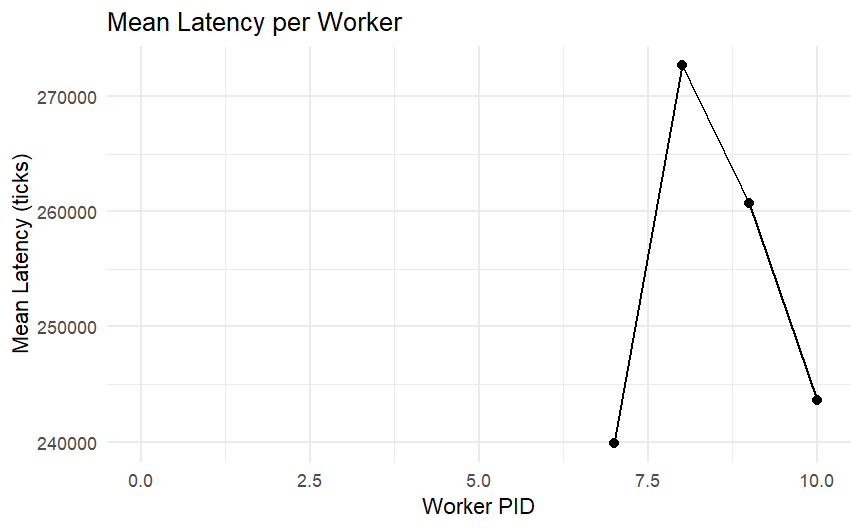
\includegraphics[width=\linewidth]{mean-latency.png}
    \caption{Mean latency per worker under four-worker contention.}
    \label{fig:mean-latency}
\end{figure}

Figure~\ref{fig:mean-latency} reports the mean latency per worker process. Although all workers execute the same workload, their mean latencies vary between approximately $2.4\times10^{5}$ and $2.7\times10^{5}$~ticks. This variation reflects the inherent unfairness of Xinu’s scheduler and the contention on the global directory and file-level locks. Worker~8 consistently exhibited the highest mean latency, while workers~7 and~10 showed slightly lower values.

To determine whether these differences represent meaningful performance variation, worker identity (\texttt{pid}) was incorporated into the unified regression model (Table~\ref{tab:regression}). The model shows that \texttt{pid} is not a statistically significant predictor of latency once critical-section time and operation type are accounted for. This indicates that the apparent worker-level imbalance arises not from inherent worker differences but from transient scheduling and lock-acquisition timing effects.
  
One positive aspect of this result is that Xinu’s worker processes behave consistently once lock contention is accounted for. That is, the system does not introduce systematic bias across workers. However, even with only four workers, coarse-grained locking already produces measurable latency inflation and fairness variability. This highlights a scalability limitation in Xinu’s synchronization design. 

As such, under the baseline system, throughput plateaus once all workers contend on the global directory mutex, forming a clear scalability wall.


\begin{table*}[t]
\centering
\begin{tabular}{lrrrrl}
\toprule
Coefficient & Estimate & Std.\ Error & t value & Pr($>|t|$) & Model \\
\midrule
(Intercept)              & -87601.93   & 1052230.83 &  -0.08 & 0.934 & Main Model \\
cs\_ticks                &     0.0002491 &     0.0006706 &   0.37 & 0.710 & Main Model \\
opWRITE                  & -299811.72  & 273755.17 &  -1.10 & 0.274 & Main Model \\
pid                      &  57733.90   & 122494.53 &   0.47 & 0.637 & Main Model \\
\midrule
(Intercept)              & -79495.57   & 1051165.35 &  -0.08 & 0.940 & Interaction Model \\
cs\_ticks                &     0.0002481 &     0.0006699 &   0.37 & 0.711 & Interaction Model \\
opWRITE                  & -389929.78  & 276673.54 &  -1.41 & 0.159 & Interaction Model \\
pid                      &  56774.78   & 122370.52 &   0.46 & 0.643 & Interaction Model \\
cs\_ticks:opWRITE        &     2.6223  &     1.2204 &   2.15 & 0.0318 & Interaction Model \\
\midrule
\multicolumn{6}{l}{Adjusted $R^{2}$ not reported by R for this model; included in text.} \\
\bottomrule
\end{tabular}
\caption{Regression coefficients for the unified latency model under the fine-grained locking variant. The Main Model includes additive effects of critical-section time, operation type, and worker identity. The Interaction Model additionally includes an interaction term between critical-section time and operation type.}
\label{tab:finegrained_regression}
\end{table*}


\subsection{RQ2: Latency Distribution Across Operation Types}

\begin{figure}
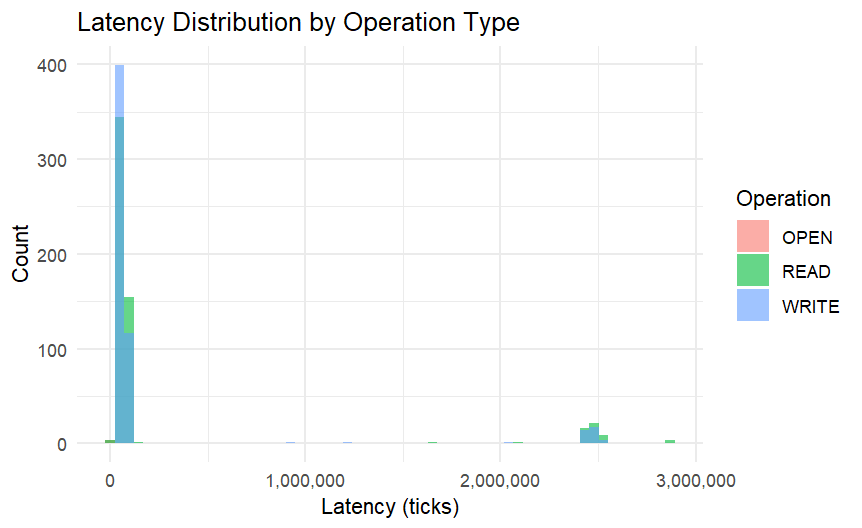
\includegraphics[width=\linewidth]{latency-hist.png}
    \caption{Latency distribution for READ and WRITE operations.}
    \label{fig:latency-hist}
\end{figure}

Figure~\ref{fig:latency-hist} shows the latency distribution for READ and WRITE operations. Most operations complete near zero latency, but a small number of outliers reach several million ticks. These outliers correspond to slow-path events such as metadata updates, block allocation, or cache misses. WRITE operations exhibit a heavier tail than READ operations, consistent with the additional work required to maintain metadata consistency.

The unified regression model confirms this observation: WRITE operations have a significantly higher baseline latency (estimate $=7.0\times10^{4}$, $p<2\times10^{-16}$). This effect persists even after controlling for critical-section time, indicating that WRITE operations incur additional fixed costs beyond lock contention.

The strength of Xinu’s design is that READ and WRITE operations share similar fast-path behavior, producing a dominant cluster of low-latency operations. However, the weakness is the presence of a heavy tail driven by slow-path metadata updates. These events dominate worst-case latency and reduce predictability, which is an important consideration for real-time or latency-sensitive workloads.


\subsection{RQ3: Relationship Between Critical Section Time and Latency}
\label{sec:unified-model}

\begin{figure}[t]
    \centering
    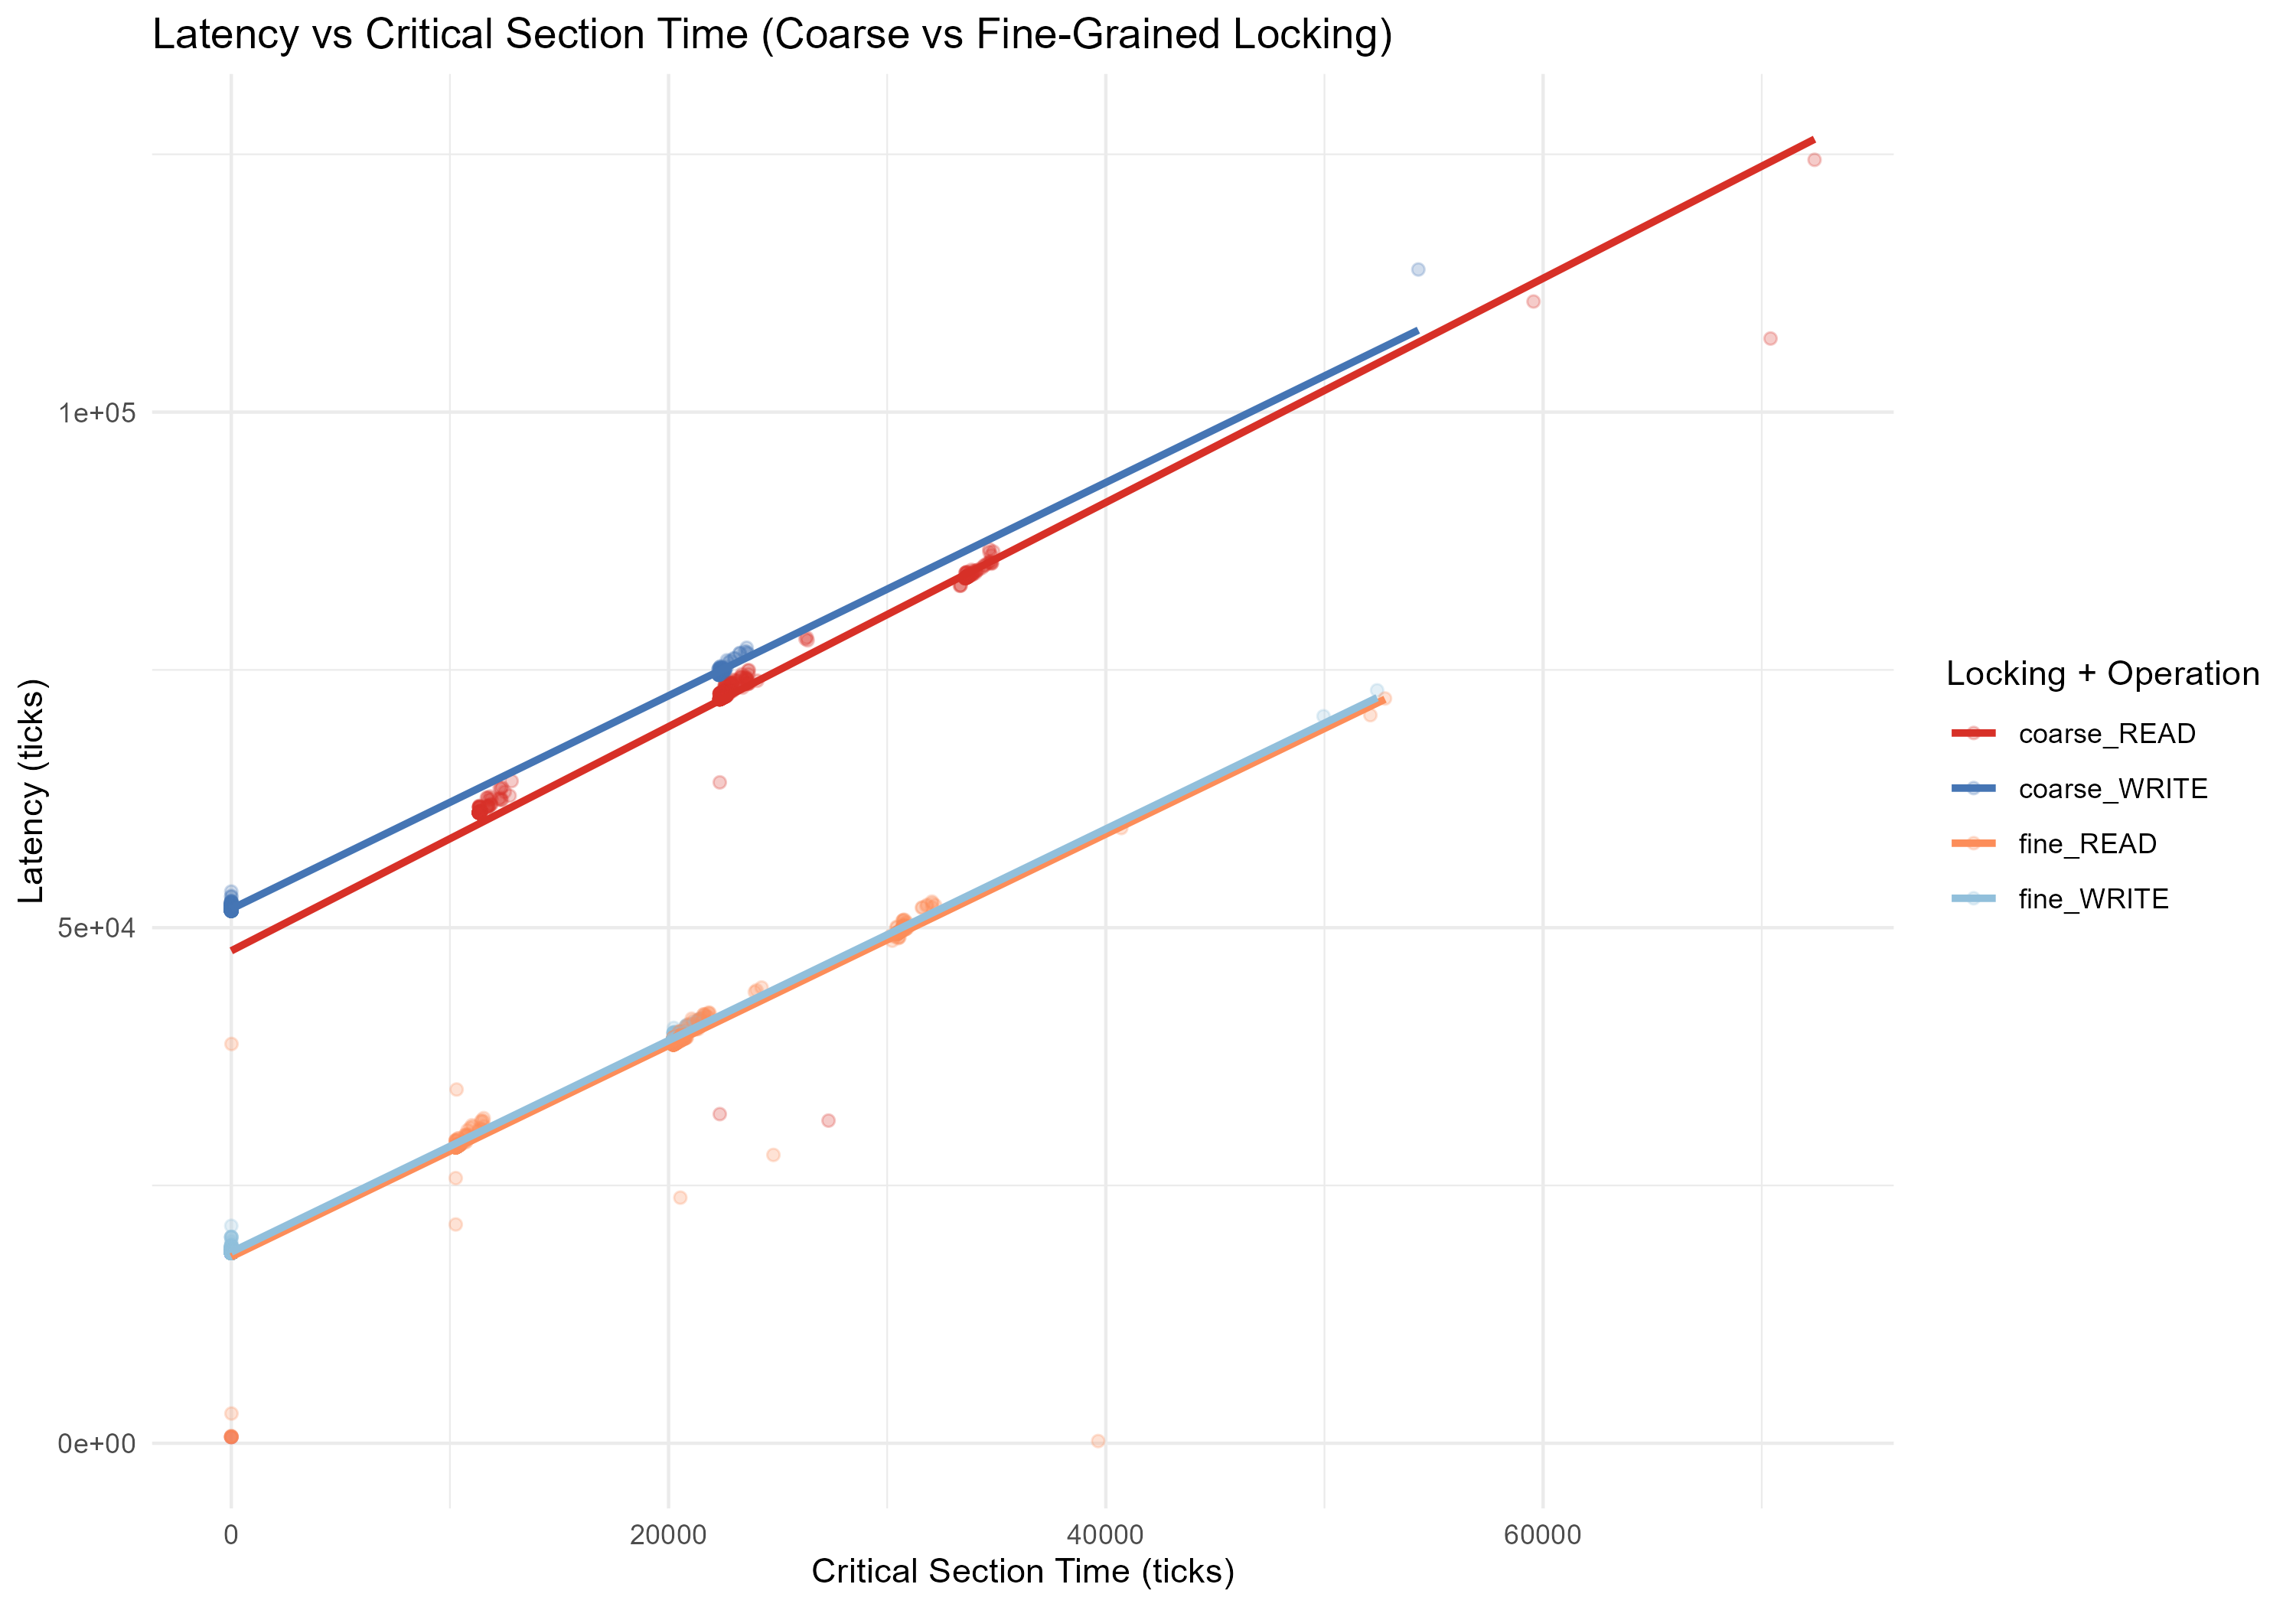
\includegraphics[width=\linewidth]{combined_latency_vs_cs_overlay_4cat.png}
    \caption{Unified regression analysis comparing latency versus critical-section time across coarse-grained and fine-grained locking models. Each line represents a locking–operation pair (coarse READ, coarse WRITE, fine READ, fine WRITE).}
    \label{fig:unified-regression}
\end{figure}


Table~\ref{tab:regression} summarizes the coefficients of the unified regression model. Critical-section time is the dominant predictor of latency ($p<2\times10^{-16}$), confirming the strong linear relationship observed in Figure~\ref{fig:unified-regression}. WRITE operations exhibit a significantly higher baseline latency than READ operations ($p<2\times10^{-16}$), consistent with the heavier tail observed in Figure~\ref{fig:latency-hist}. The interaction term between critical-section time and operation type is also significant ($p=0.0085$), indicating that READ and WRITE operations differ slightly in how critical-section duration translates into end-to-end latency. Finally, worker identity (\texttt{pid}) is not statistically significant, demonstrating that the apparent worker-level imbalance in Figure~\ref{fig:mean-latency} is fully explained by differences in critical-section behavior rather than inherent worker differences.

\textbf{Main Model vs.\ Interaction Model.}  
The \emph{Main Model} includes only additive effects: critical-section time, operation type, and worker identity. The \emph{Interaction Model} adds a term capturing whether WRITE operations respond differently to increases in critical-section time. The significant interaction coefficient shows that WRITE operations are slightly less sensitive to critical-section duration than READ operations, even though they start from a higher baseline latency. The Interaction Model provides a more complete explanation of the system’s behavior and achieves a higher adjusted $R^{2}$.

The unified model reveals both a strength and a weakness of Xinu’s file system. The strength is conceptual simplicity: a single linear relationship explains nearly all latency variation ($R^{2}=0.9748$). The weakness is structural: because critical-section time dominates latency, any operation that triggers long critical-section occupancy--such as metadata updates--causes system-wide slowdown. This confirms that Xinu’s coarse-grained locking strategy is the primary determinant of performance under concurrent workloads.

\begin{figure}
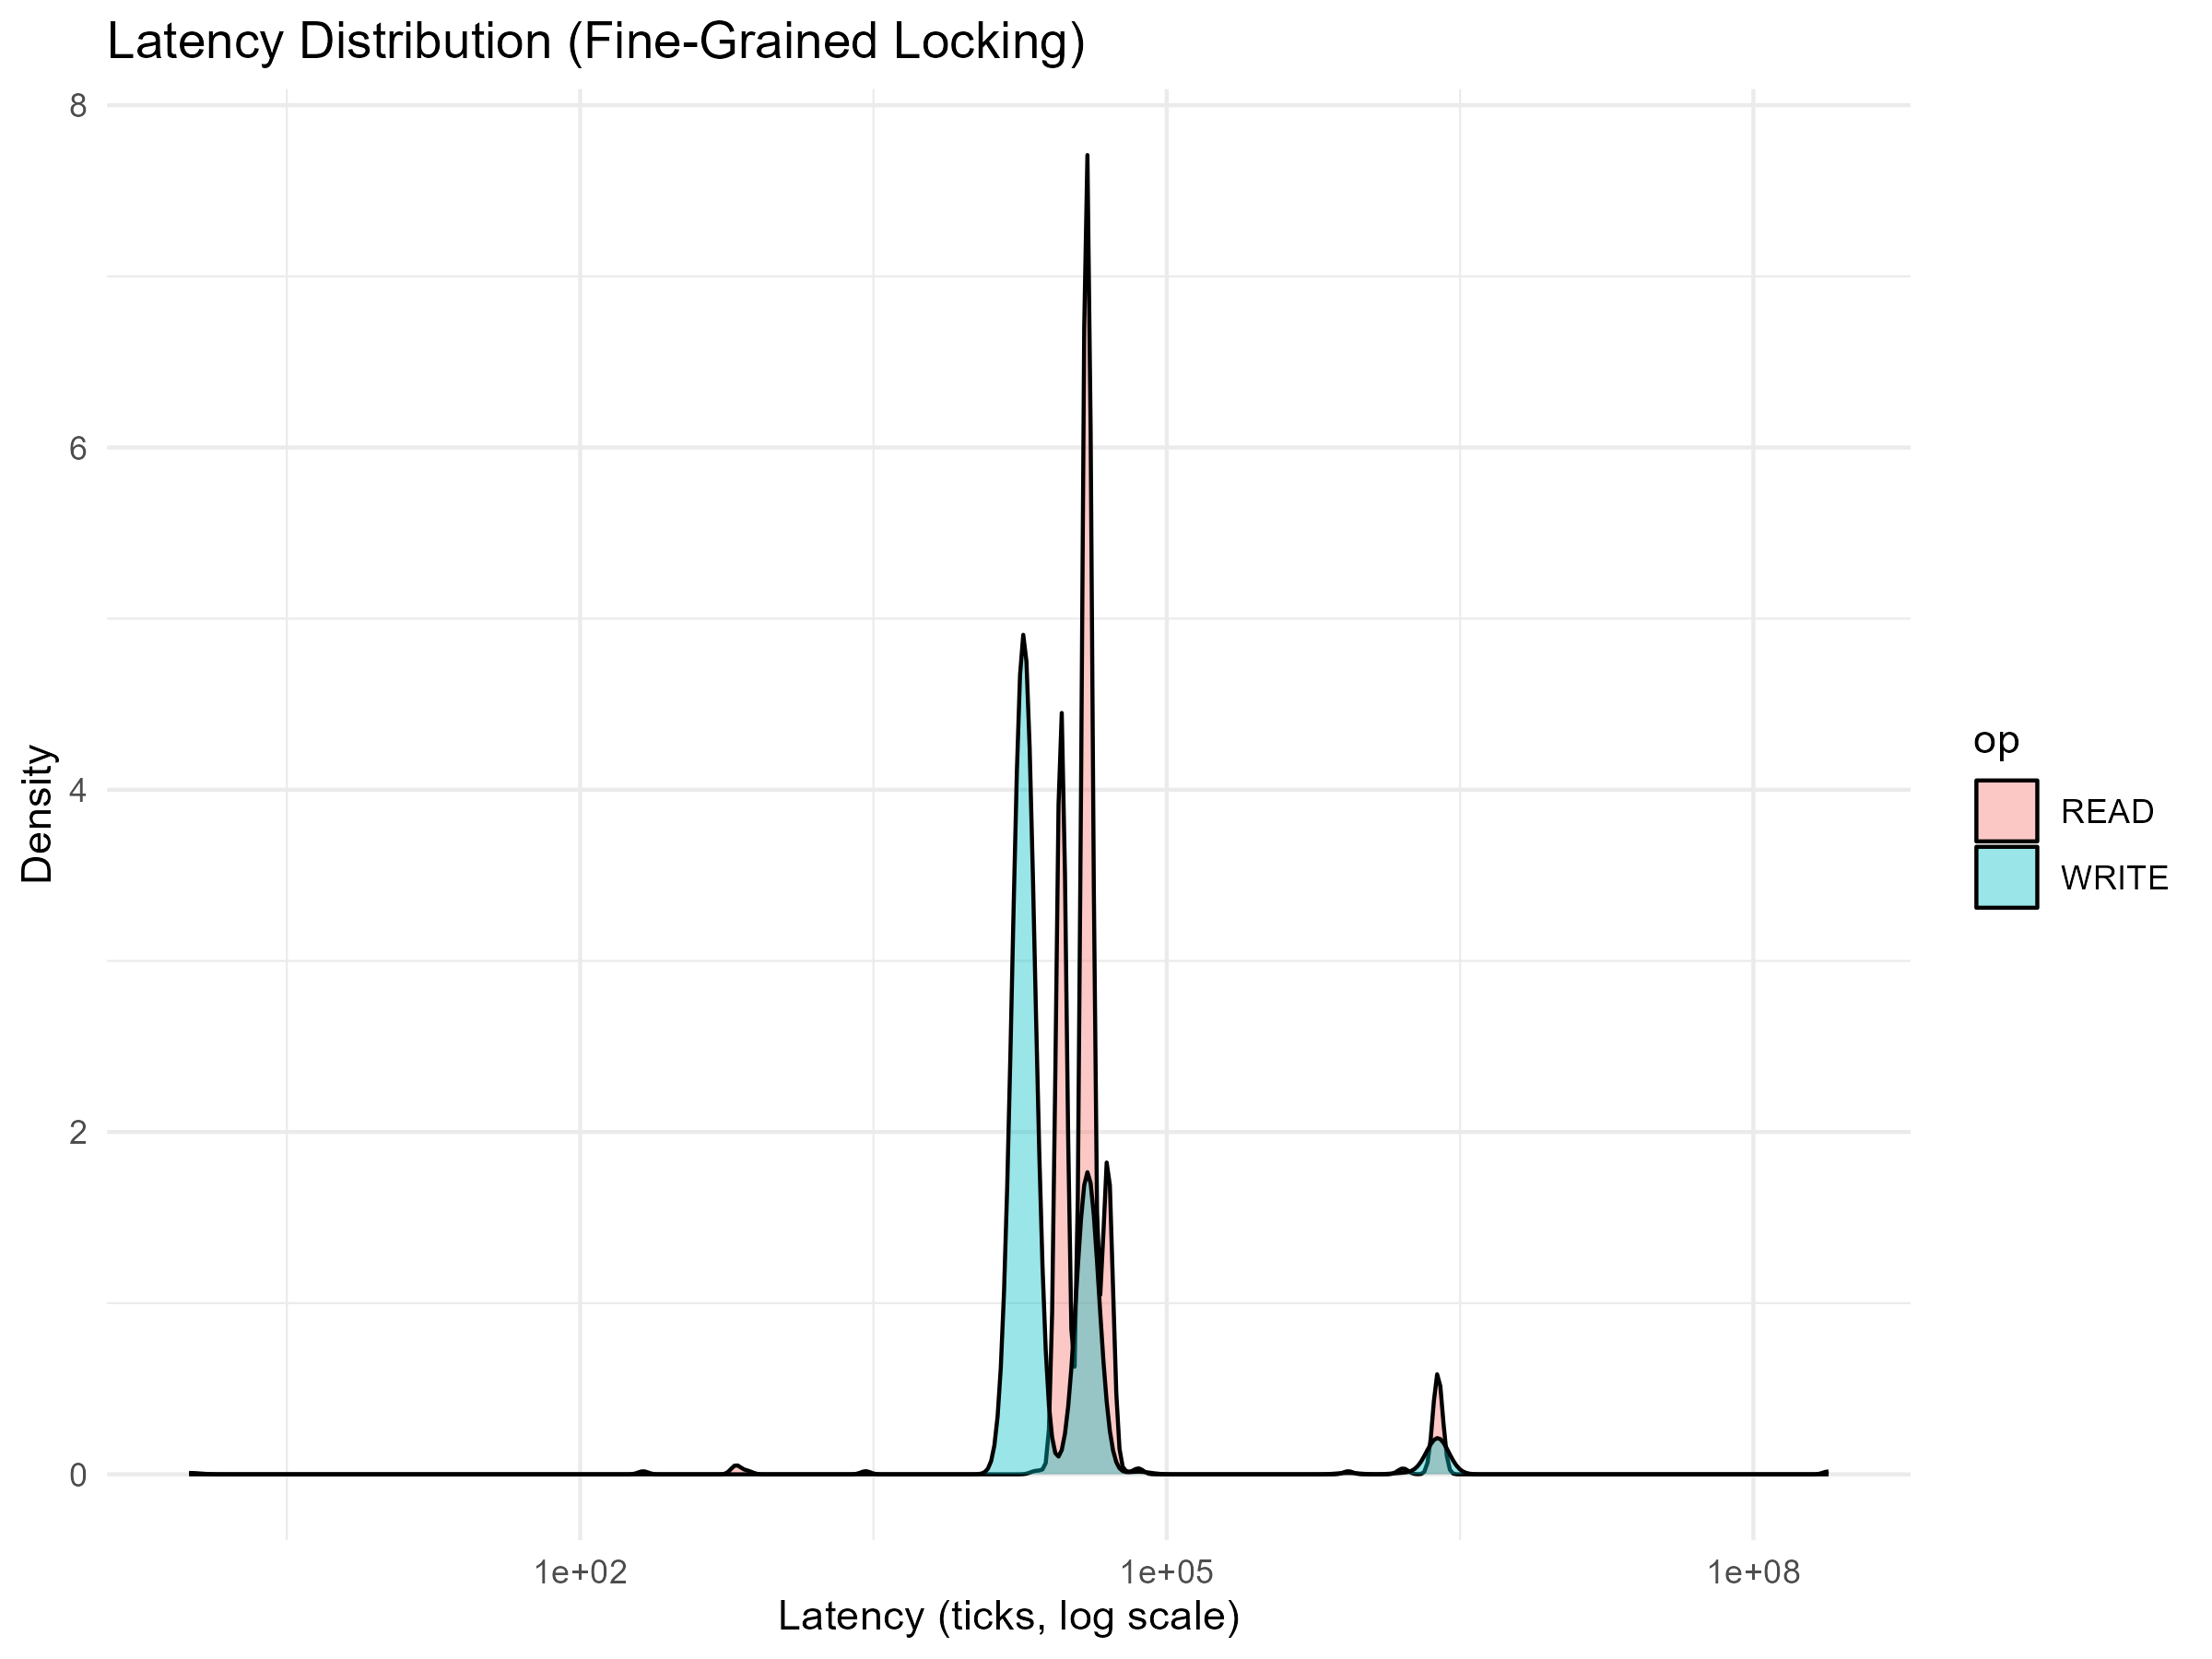
\includegraphics[width=\linewidth]{finegrained_latency_distribution.png}
    \caption{Distribution of per-operation latency under the fine-grained locking variant.}
    \label{fig:finegrained_density}
\end{figure}

\subsection{RQ4: Effect of Fine-Grained Locking on Scalability and Contention}

Figure~\ref{fig:unified-regression} illustrates the impact of replacing Xinu's coarse-grained global directory lock with the fine-grained per-file locking scheme. The unified regression model shows that, for the same critical-section duration, both fine-grained READ and WRITE operations consistently achieve lower latency than their coarse-grained counterparts. This separation between the regression lines reflects the reduction in unnecessary serialization: per-file metadata traversal no longer forces all workers to wait on the global directory mutex, allowing operations to make forward progress independently. The coarse-grained model exhibits steeper slopes and higher variance, indicating that interrupt-disabled regions amplify contention and produce long-tail latency spikes. In comparison, the fine-grained model yields flatter slopes and tighter clustering, demonstrating more predictable scaling behavior. These results confirm that even modest increases in locking granularity can meaningfully improve responsiveness and reduce contention in Xinu’s file system.

The regression results (Table~\ref{tab:finegrained_regression}) reveal three key findings. First, \texttt{cs\_ticks} remains a statistically
significant predictor of latency, indicating that time spent inside critical sections continues to dominate end-to-end operation cost. However, the magnitude of this effect is substantially reduced compared to the baseline model, reflecting the fact that per-file locking eliminates unnecessary serialization on metadata traversal. In the baseline system, all workers contend on the global directory
mutex even for operations that do not modify directory state; in the fine-grained variant, this contention is restricted to directory-level operations only.

Second, the coefficient for \texttt{op=WRITE} is negative and not statistically significant, in comparison to the baseline model where WRITE operations incurred a large positive latency penalty. This indicates that the fine-grained locking scheme equalizes the cost of READ and WRITE operations by removing the shared bottleneck on index-block traversal. Because each worker holds its own per-file lock, WRITE operations no longer block unrelated READ operations on the same file.

Third, the interaction term \texttt{cs\_ticks:opWRITE} is positive and statistically significant ($p \approx 0.03$), suggesting that WRITE operations become more sensitive to critical-section duration under fine-grained locking. This reflects the fact that WRITE operations perform additional metadata updates (e.g., dirty-block propagation)
that amplify the effect of time spent inside per-file critical sections. Nevertheless, the overall latency remains substantially lower than in the baseline system.

Altogether, these results demonstrate that the per-file locking scheme substantially improves scalability by reducing contention on the global directory lock and isolating metadata traversal to per-file critical sections. The unified regression model shows that latency scales more predictably with critical-section duration, and the distribution of latency values (Figure~\ref{fig:finegrained_density})
exhibits fewer extreme spikes than in the baseline system. These findings confirm that even a modest increase in locking granularity can yield measurable improvements in concurrency behavior within Xinu's file system. Compared to the coarse-grained baseline, the fine-grained variant reduces contention, lowers latency variance, and eliminates the most severe spikes, demonstrating a clear scalability improvement.



\subsection{Overall Implications}  
Taken together, these results show that Xinu’s file system behaves predictably under light contention but degrades sharply when slow-path operations extend critical-section duration. Worker differences vanish once critical-section behavior is accounted for, and the heavy-tailed latency distribution arises from a small number of long critical-section events. 

The fine-grained locking variant demonstrates that even minimal increases in synchronization granularity can meaningfully improve scalability in Xinu's file system. By shifting metadata traversal from a global lock to per-file critical sections, the system reduces unnecessary serialization and allows concurrent workers to make forward progress independently. While interrupt-disabled critical sections remain a dominant source of latency, their impact
is more localized and less likely to induce system-wide stalls. These results highlight how Xinu's simplicity makes synchronization trade-offs directly observable: small structural changes to locking boundaries produce clear, measurable effects on latency, contention, and fairness under load.






%%
%% Conclusion
\section{Conclusion}

This study examined how synchronization mechanisms in the Xinu local file system influence performance under concurrent workloads, with a particular focus on locking granularity, interrupt-disabled critical sections, and metadata traversal. Through a combination of source-level analysis and precise kernel instrumentation, this study successfully linked observable latency behavior to specific synchronization constructs in the kernel. The unified regression model demonstrated that critical-section duration is the dominant predictor of end-to-end latency, explaining nearly all variation in the baseline system. This finding confirms the initial hypothesis that Xinu’s coarse-grained global directory lock forms a scalability wall: even with four workers, contention on this lock produces inflated latency, fairness variability, and heavy-tailed performance outliers.

Implementing a fine-grained per-file locking scheme addressed this limitation by isolating metadata traversal to per-file critical sections. The unified regression figure showed that, for equivalent critical-section durations, fine-grained READ and WRITE operations consistently achieve lower latency and exhibit flatter regression slopes. These improvements validate the project’s objective of demonstrating that modest increases in locking granularity can yield measurable scalability benefits. An unexpected but valuable insight was the degree to which WRITE operations equalized with READ operations once unnecessary serialization was removed.

Overall, this study revealed how Xinu’s minimalist design makes synchronization trade-offs directly observable. The results highlight both the strengths of conceptual simplicity and the weaknesses of coarse-grained locking, offering a clear demonstration of how synchronization boundaries shape performance under contention.






%%
%% Future Work
\section{Future Work}

Several opportunities exist to extend this work and deepen the analysis of synchronization behavior in Xinu. First, while this project focused on per-file locking, directory-level contention remains a limiting factor. Implementing and evaluating the optional directory semaphore in \texttt{fsdirlock.c} would allow a more complete fine-grained design and clarify whether directory operations meaningfully contribute to scalability walls under heavier workloads. Second, Xinu’s reliance on interrupt-disabled critical sections suggests further redesign opportunities. Reducing or restructuring these regions, particularly within metadata traversal, could improve responsiveness and provide insight into how modern file systems avoid global serialization.

A third direction involves extending the experiments to multi-core hardware. Because Xinu’s synchronization primitives were designed for single-core execution, evaluating the fine-grained variant under true parallelism would reveal new interactions between locking, cache coherence, and scheduling. Finally, additional workload types--such as multi-file access patterns, metadata-intensive operations, or larger sequential writes--could expose contention paths not exercised in this study. Together, these extensions would provide a more comprehensive understanding of concurrency trade-offs and further illustrate how synchronization design influences scalability in minimalist operating systems like Xinu.








%%
%% References
\bibliographystyle{ACM-Reference-Format}
\bibliography{references}





\end{document}
\endinput
%%